\section{Problem 8}

\subsection{MATLAB code}

\begin{lstlisting}
%% Problem 9a

% correlationExperiments.m
%
% Experiment with properties of pseudorandom sequences.


clear;clc;
addpath("research/toolbox/")
%----- Setup
nStages = 10;                 % Number of stages in LFSR
Tc = 1e-3/1023;               % Chip interval in seconds
delChip = 3/217;              % Sampling interval in chips
delOffset  = 0;               % Offset of first sample
delt = delChip*Tc;            % Sampling interval in seconds
fs = 1/delt;                  % Sampling frequency in Hz
Np = 2^nStages - 1;           % Period of the sequence in chips
Nr = 20;                      % Number of repetitions of the sequence
Ns = round(Nr*Np/delChip);    % Number of samples of the sequence 

N = 10000;
varVec = zeros(N,1);
for i=1:N
    % codeType:
    % rand ---- Sequence derived from Matlab randn function
    % pi ------ Sequence derived from the digits of pi
    % mseq ---- Maximal-length sequence with n = nStages
    codeType = 'rand';
    
    %----- Generate codes
    X1 = zeros(Np,1);
    X2 = zeros(Np,1);
    if(strcmp(codeType,'rand'))
      X1 = sign(sign(randn(Np,1)) + 0.1);
      X2 = sign(sign(randn(Np,1)) + 0.1);
    elseif(strcmp(codeType,'pi'))
      [sPi,vPi] = pi2str(2*Np);
      X1 = vPi(1:Np) >= 5;
      X1 = 2*X1 - 1;
      X2 = vPi(Np+1:2*Np) >= 5;
      X2 = 2*X2 - 1;
    elseif(strcmp(codeType,'mseq'))
    ciVec1 = [9, 4]';  
    ciVec2 = [9, 2]';
    a0Vec1 = [1;zeros(nStages-1,1)];
    a0Vec2 = ones(nStages,1);
    X1 = generateLfsrSequence(nStages,ciVec1,a0Vec1);
    X2 = generateLfsrSequence(nStages,ciVec2,a0Vec2);
    X1 = 2*X1 - 1;
    X2 = 2*X2 - 1;
    else
      error('Unrecognized code type');
    end
    
    %----- Compute the sequence crosscorrelation
    [Rseq12,iiVecSeq] = ccorr(X1,X2);
    index = find(iiVecSeq==0);
    crosscorrVec(i) = Rseq12(index);
end

% The problem asks about the variance of the cross-correlation at k=0
var(crosscorrVec)
\end{lstlisting}

\begin{lstlisting}
%% Problem 9b

% correlationExperiments.m
%
% Experiment with properties of pseudorandom sequences.


clear;clc; format short
addpath("research/toolbox/")
%----- Setup
nStages = 10;                 % Number of stages in LFSR
Tc = 1e-3/1023;               % Chip interval in seconds
delChip = 3/217;              % Sampling interval in chips
delOffset  = 0;               % Offset of first sample
delt = delChip*Tc;            % Sampling interval in seconds
fs = 1/delt;                  % Sampling frequency in Hz
Np = 2^nStages - 1;           % Period of the sequence in chips
Nr = 20;                      % Number of repetitions of the sequence
Ns = round(Nr*Np/delChip);    % Number of samples of the sequence 

N = 6;
varVec = zeros(N,1);
for i=1:N
    ciVec1 = [
        [10, 9, 8, 5]',...  
        [10, 9, 7, 6]',...
        [10, 9, 7, 3]',...
        [10, 9, 6, 1]',...
        [10, 9, 5, 2]',...
        [10, 9, 4, 2]'
    ];
    ciVec2 = [
        [10, 9, 8, 7, 5, 4]',...  
        [10, 9, 8, 7, 4, 1]',...
        [10, 9, 8, 7, 3, 2]',...
        [10, 9, 8, 6, 5, 1]',...
        [10, 9, 8, 6, 4, 2]',...
        [10, 9, 8, 6, 4, 2]'  
    ];
    a0Vec1 = [1;zeros(nStages-1,1)];
    a0Vec2 = ones(nStages,1);
    X1 = generateLfsrSequence(nStages,ciVec1(:,i),a0Vec1);
    X2 = generateLfsrSequence(nStages,ciVec2(:,i),a0Vec2);
    X1 = 2*X1 - 1;
    X2 = 2*X2 - 1;
    %----- Compute the sequence crosscorrelation
    [Rseq12,iiVecSeq] = ccorr(X1,X2);
    
    bound_crosscorrVec(i) = max(Rseq12);

    %----- Compute the sequence autocorrelation
    [Rseq11,iiVecSeq] = ccorr(X1,X1);
    index = find(iiVecSeq==0);
    autocorrVec(i) = Rseq11(index);
end

% The value of the autocorr at k=0 ~ (N-1)
autocorrVec

% The bound of the cross-correlation >= sqrt(N)
bound_crosscorrVec
\end{lstlisting}

\begin{lstlisting}
%% Problem 9c

clear;clc;close all
addpath("research/toolbox/")
%----- Setup
nStages = 10;                 % Number of stages in LFSR
Tc = 1e-3/1023;               % Chip interval in seconds
delChip = 3/217;              % Sampling interval in chips
delOffset  = 0;               % Offset of first sample
delt = delChip*Tc;            % Sampling interval in seconds
fs = 1/delt;                  % Sampling frequency in Hz
Np = 2^nStages - 1;           % Period of the sequence in chips
Nr = 20;                      % Number of repetitions of the sequence
Ns = round(Nr*Np/delChip);    % Number of samples of the sequence 
% codeType:
% rand ---- Sequence derived from Matlab randn function
% pi ------ Sequence derived from the digits of pi
% mseq ---- Maximal-length sequence with n = nStages
codeType = 'pi'; % Change this variable to see the different results

%----- Generate codes
X1 = zeros(Np,1);
X2 = zeros(Np,1);
if(strcmp(codeType,'rand'))
  X1 = sign(sign(randn(Np,1)) + 0.1);
  X2 = sign(sign(randn(Np,1)) + 0.1);
elseif(strcmp(codeType,'pi'))
  [sPi,vPi] = pi2str(2*Np);
  X1 = vPi(1:Np) >= 5;
  X1 = 2*X1 - 1;
  X2 = vPi(Np+1:2*Np) >= 5;
  X2 = 2*X2 - 1;
elseif(strcmp(codeType,'mseq'))
ciVec1 = [9, 4]';  
ciVec2 = [9, 2]';
a0Vec1 = [1;zeros(nStages-1,1)];
a0Vec2 = ones(nStages,1);
X1 = generateLfsrSequence(nStages,ciVec1,a0Vec1);
X2 = generateLfsrSequence(nStages,ciVec2,a0Vec2);
X1 = 2*X1 - 1;
X2 = 2*X2 - 1;
else
  error('Unrecognized code type');
end

%----- Oversample code
X1os = oversampleSpreadingCode(X1,delChip,delOffset,Ns,Np);
X2os = oversampleSpreadingCode(X2,delChip,delOffset,Ns,Np);

%----- Compute autocorrelation 
[R1,iiVec] = ccorr(X1os,X1os);
[R2,iiVec] = ccorr(X2os,X2os);

%----- Compute crosscorrelation 
[R12,iiVec] = ccorr(X1os,X2os);

ratio = max(R1)/max(R12)

%----- Compute power spectra
% The scaling here ensures that sum(Si*delf) = 1 W, as expected, for i = 1, 2.
S1 = abs(delt*fft(X1os)).^2/(Ns*delt);
S2 = abs(delt*fft(X2os)).^2/(Ns*delt);
S12 = abs(delt*fft(R12)).^2/(Ns*delt);
delf = 1/(delt*Ns);
fVec = [0:Ns-1]'*(delf);

%----- Scale for 1-Hz delf for plotting
% We'll present the power spectra in units of dBW/Hz, so we need to scale
% the spectra so that they match a delf = 1 Hz frequency spacing.
S1 = S1*delf;
S2 = S2*delf;
S12 = S12*delf;

%----- Plot
figure(1);clf;
subplot(211)
plot(iiVec,R1/Ns);
grid on;
ylabel('R_{X1}');
title('X1 and X2 autocorrelation')
subplot(212)
plot(iiVec,R2/Ns);
grid on;
ylabel('R_{X2}');
xlabel('Lag (samples)');
figure(2);clf;
plot(iiVec,R12/Ns);
title('X1 and X2 crosscorrelation')
xlabel('Lag (samples)');
grid on;
ylabel('R_{X1,X2}');
figure(3);clf;
subplot(211)
plot(fVec/1e3,10*log10(S1));
grid on;
xlim([0 30]);
ylim([-100,0]);
title('X1 and X2 power spectral densities')
ylabel('S_{X1}(f) (dBW/Hz)');
subplot(212)
plot(fVec/1e3,10*log10(S2));
grid on;
xlim([0 30]);
ylim([-100,0]);
ylabel('S_{X2}(f) (dBW/Hz)');
xlabel('Frequency (kHz)');
\end{lstlisting}


\subsection{Results}

\subsubsection{Item a}

The result verifies the claim

\subsubsection{Item b}

The result verifies the claim

\subsubsection{Item c}

\begin{figure}[H]
	\centering
	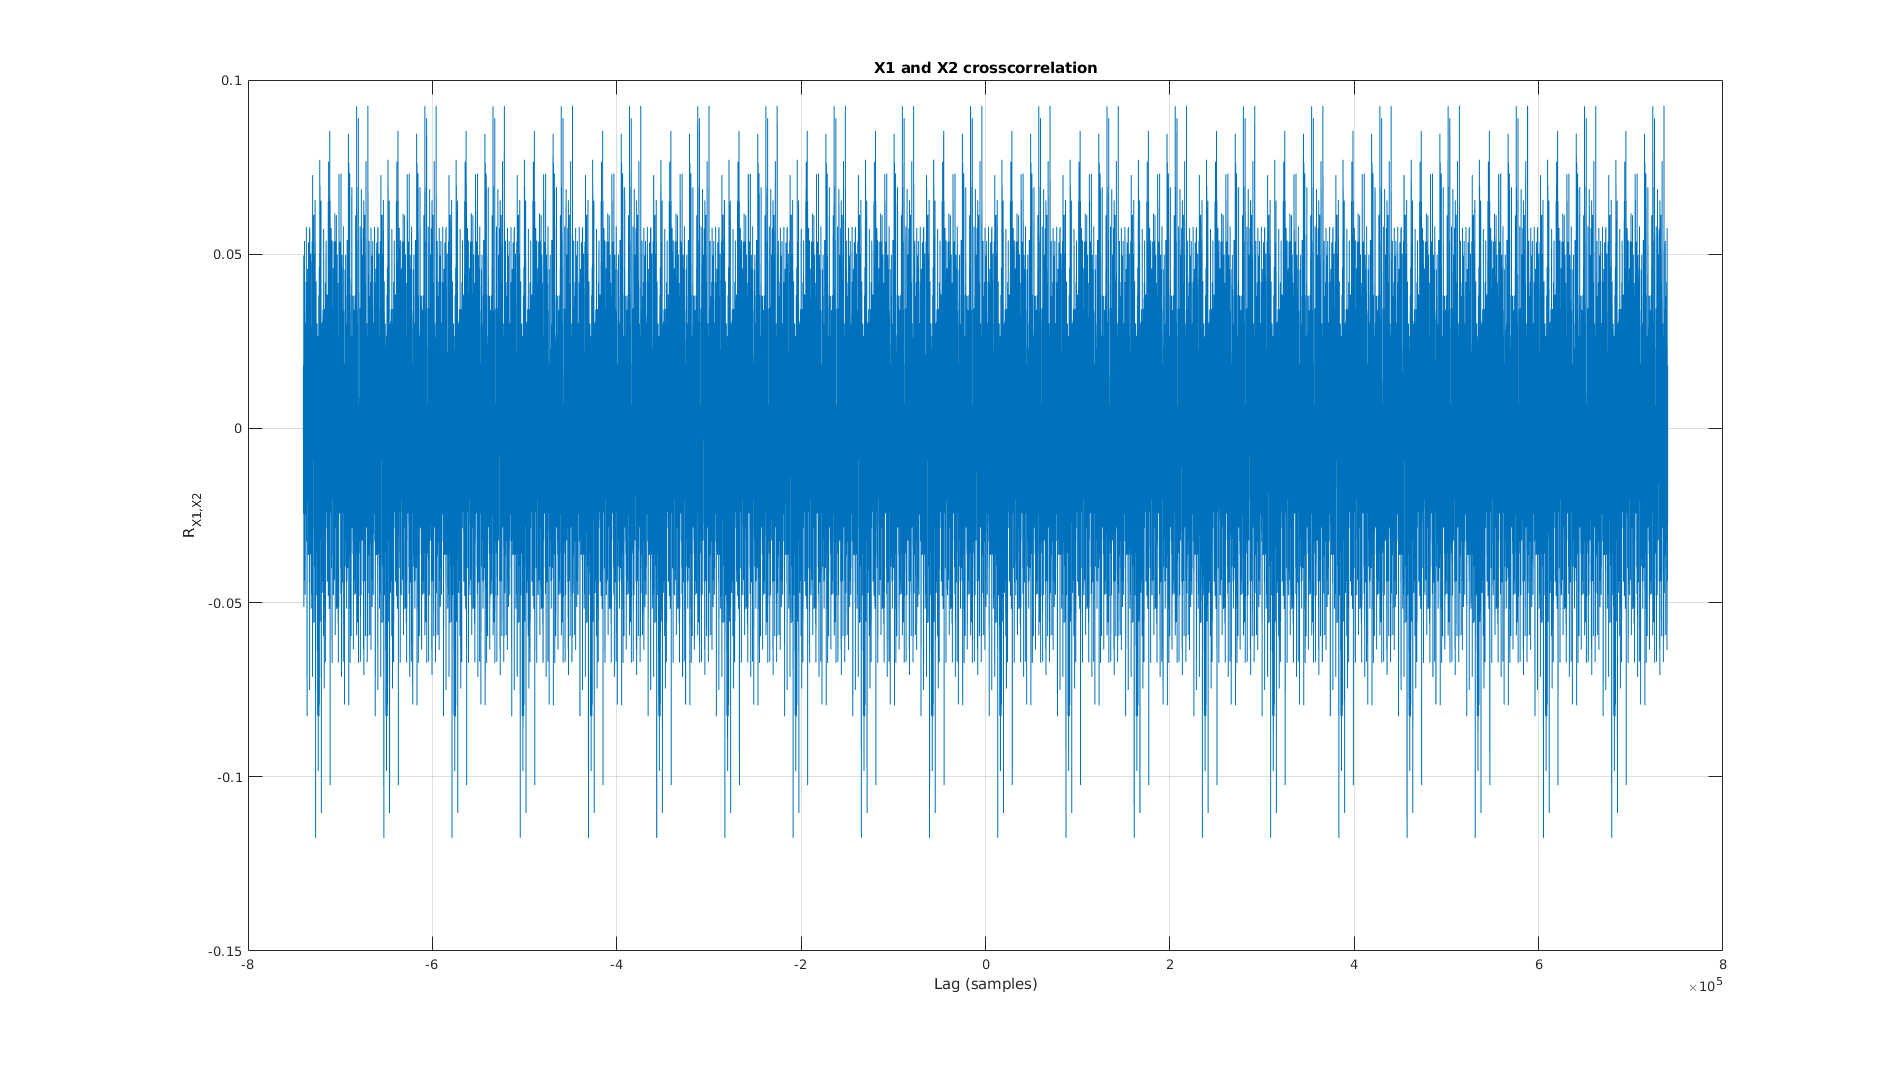
\includegraphics[width=0.9\textwidth]{figs/ex8_crosscorr_rand.png}
	\caption{Crosscorrelation of X1 and X2 for the \'rand\' case.}
	\label{fig:ex8_crosscorr_rand}
\end{figure}

\begin{figure}[H]
	\centering
	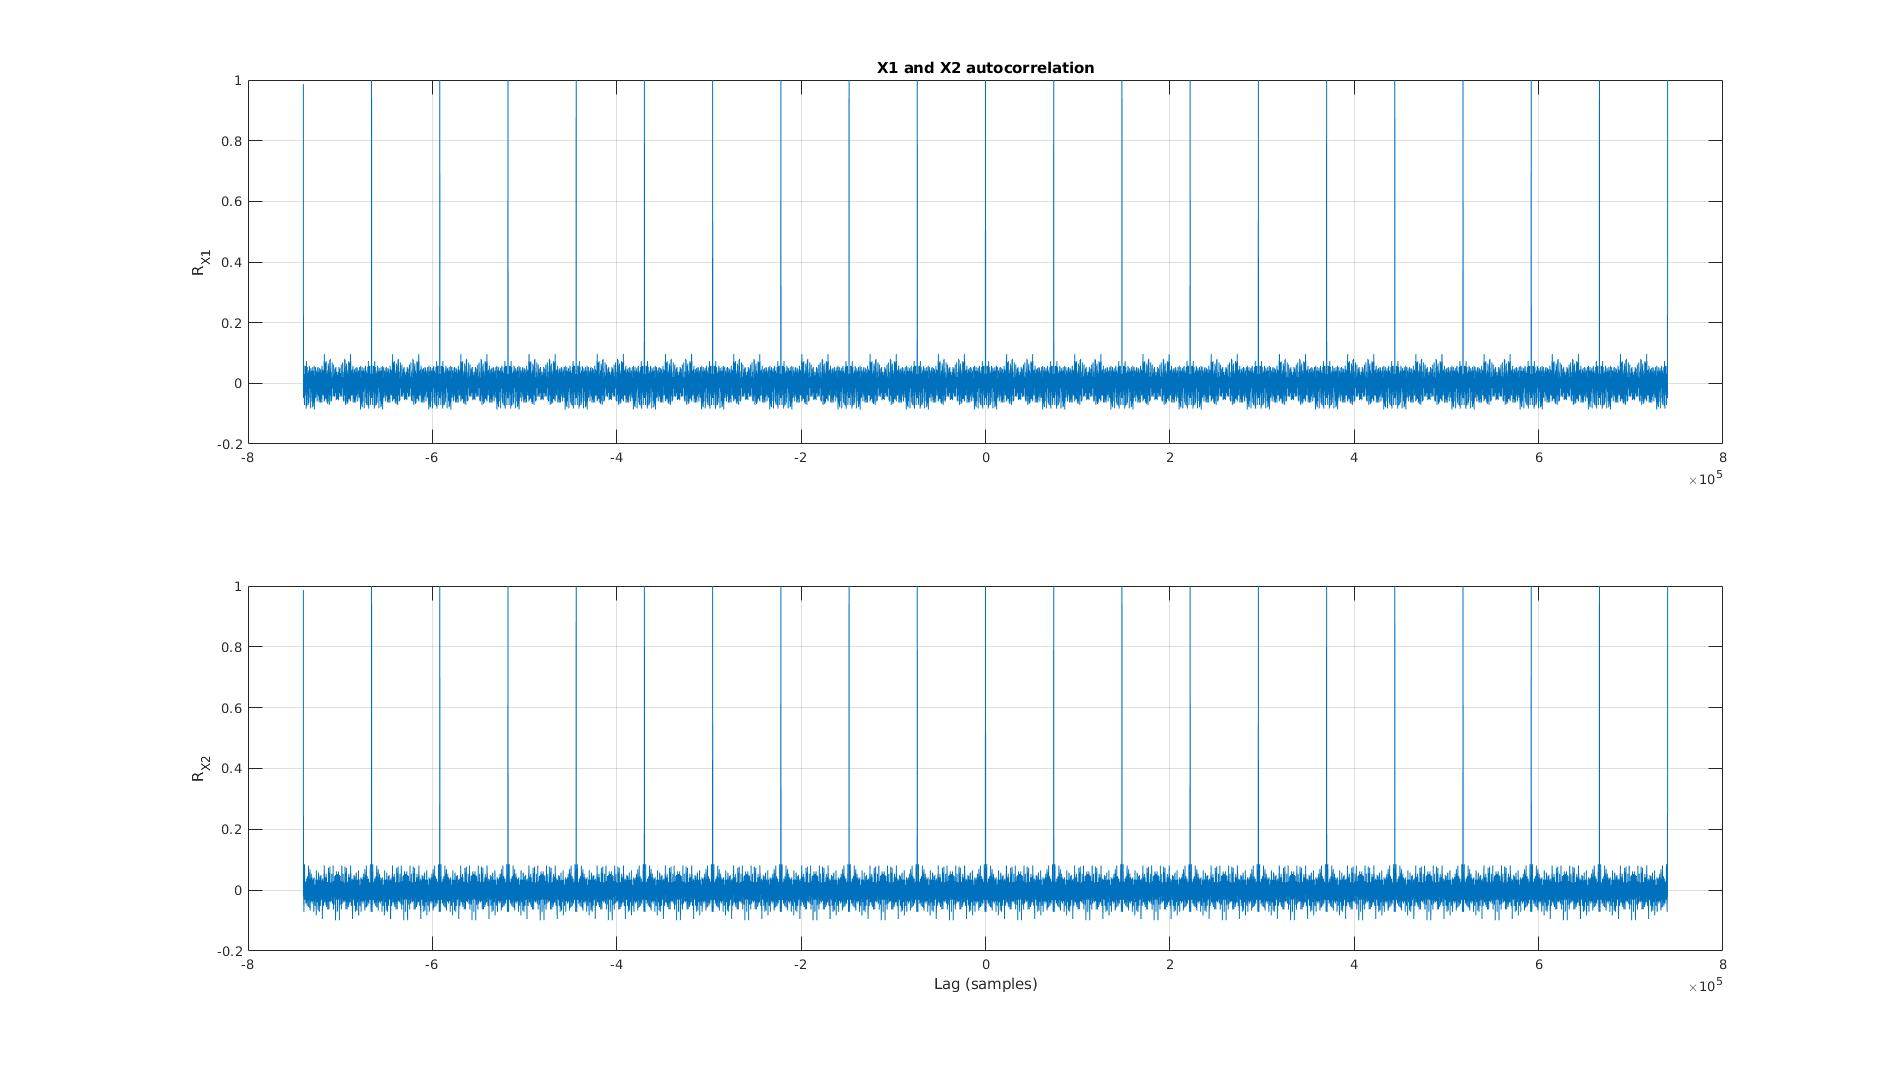
\includegraphics[width=0.9\textwidth]{figs/ex8_autocorr_rand.png}
	\caption{Autocorrelation of X1 and X2 for the 'rand' case.}
	\label{fig:ex8_autocorr_rand}
\end{figure}

\begin{figure}[H]
	\centering
	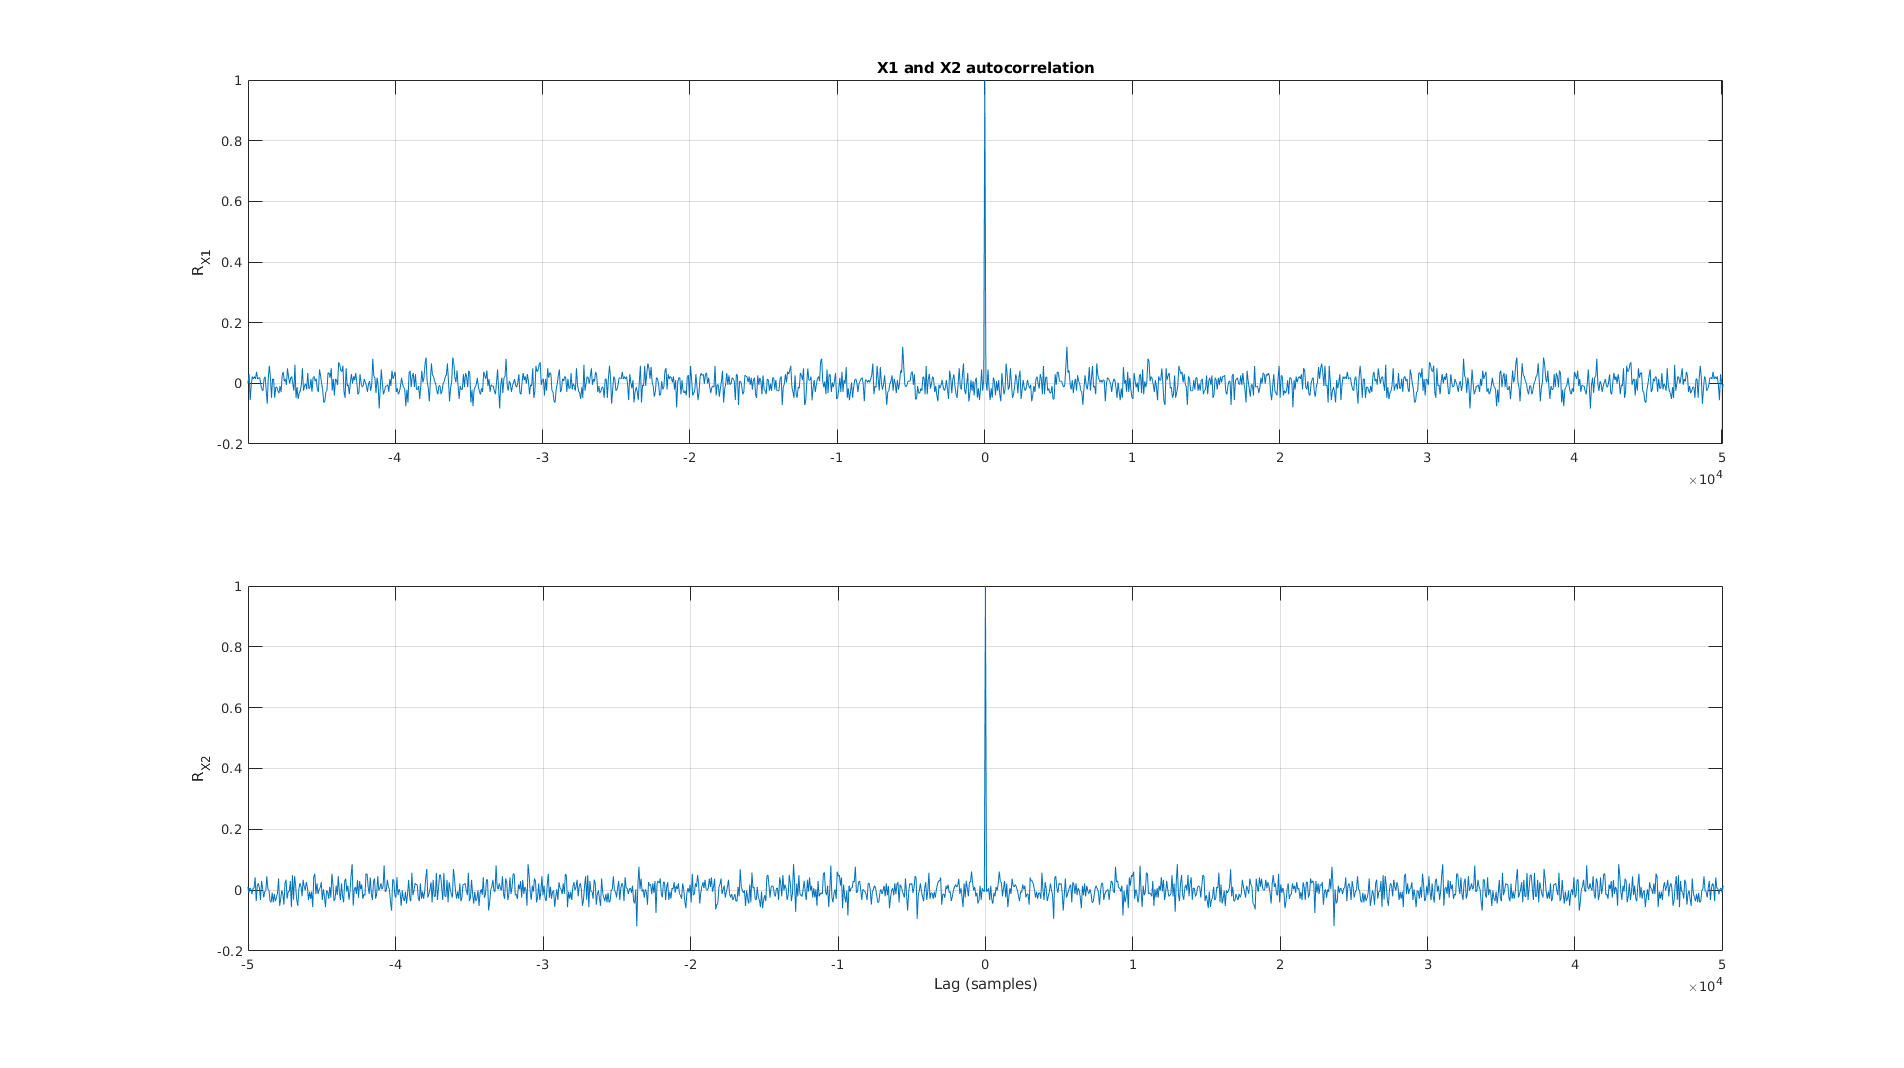
\includegraphics[width=0.9\textwidth]{figs/ex8_autocorr_zoomed_rand.png}
	\caption{Zoomed autocorrelation of X1 and X2 for the 'rand' case.}
	\label{fig:ex8_autocorr_zoomed_rand}
\end{figure}

The ratio of the maximum of $R_X(\tau)$ to the maximum of $R_{X1,X2}(\tau)$ is
11.54 for the case where we work with 'rand' method.

\begin{figure}[H]
	\centering
	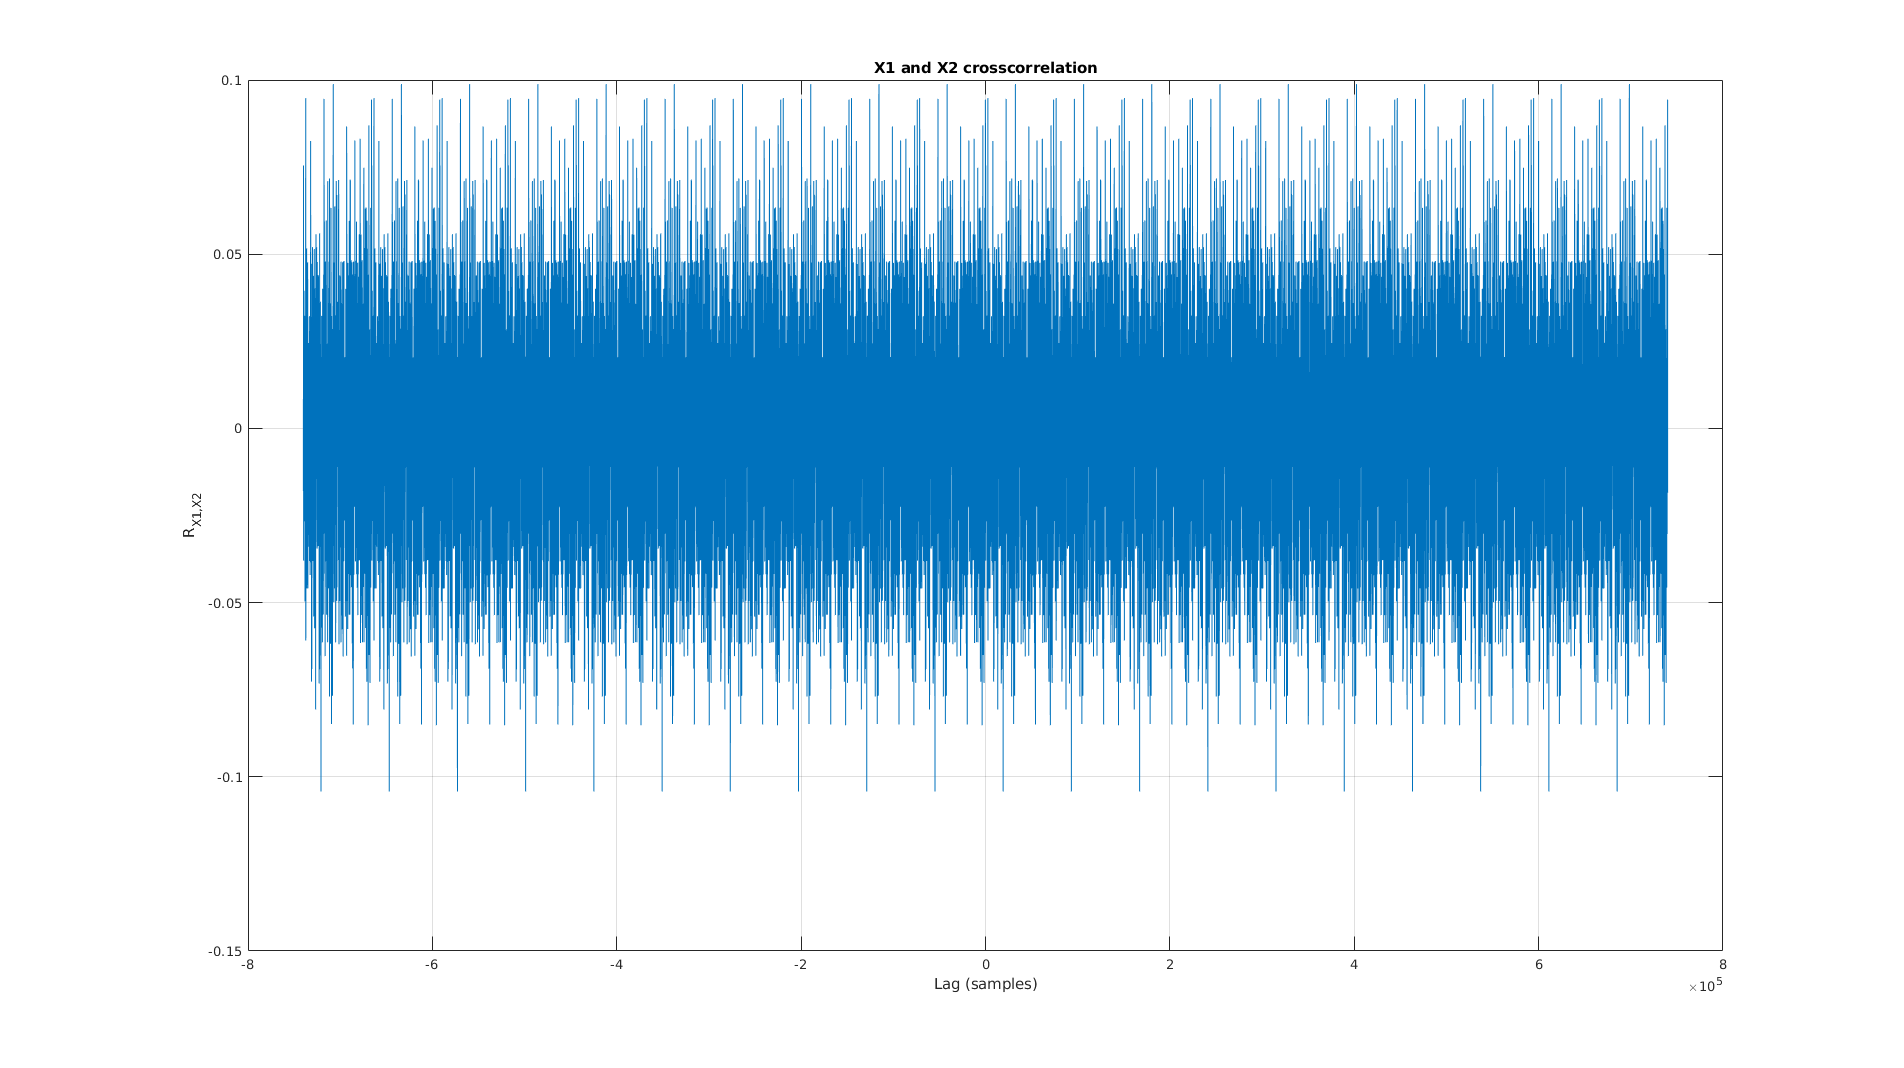
\includegraphics[width=0.9\textwidth]{figs/ex8_crosscorr_pi.png}
	\caption{Crosscorrelation of X1 and X2 for the 'pi' case.}
	\label{fig:ex8_crosscorr_pi}
\end{figure}

\begin{figure}[H]
	\centering
	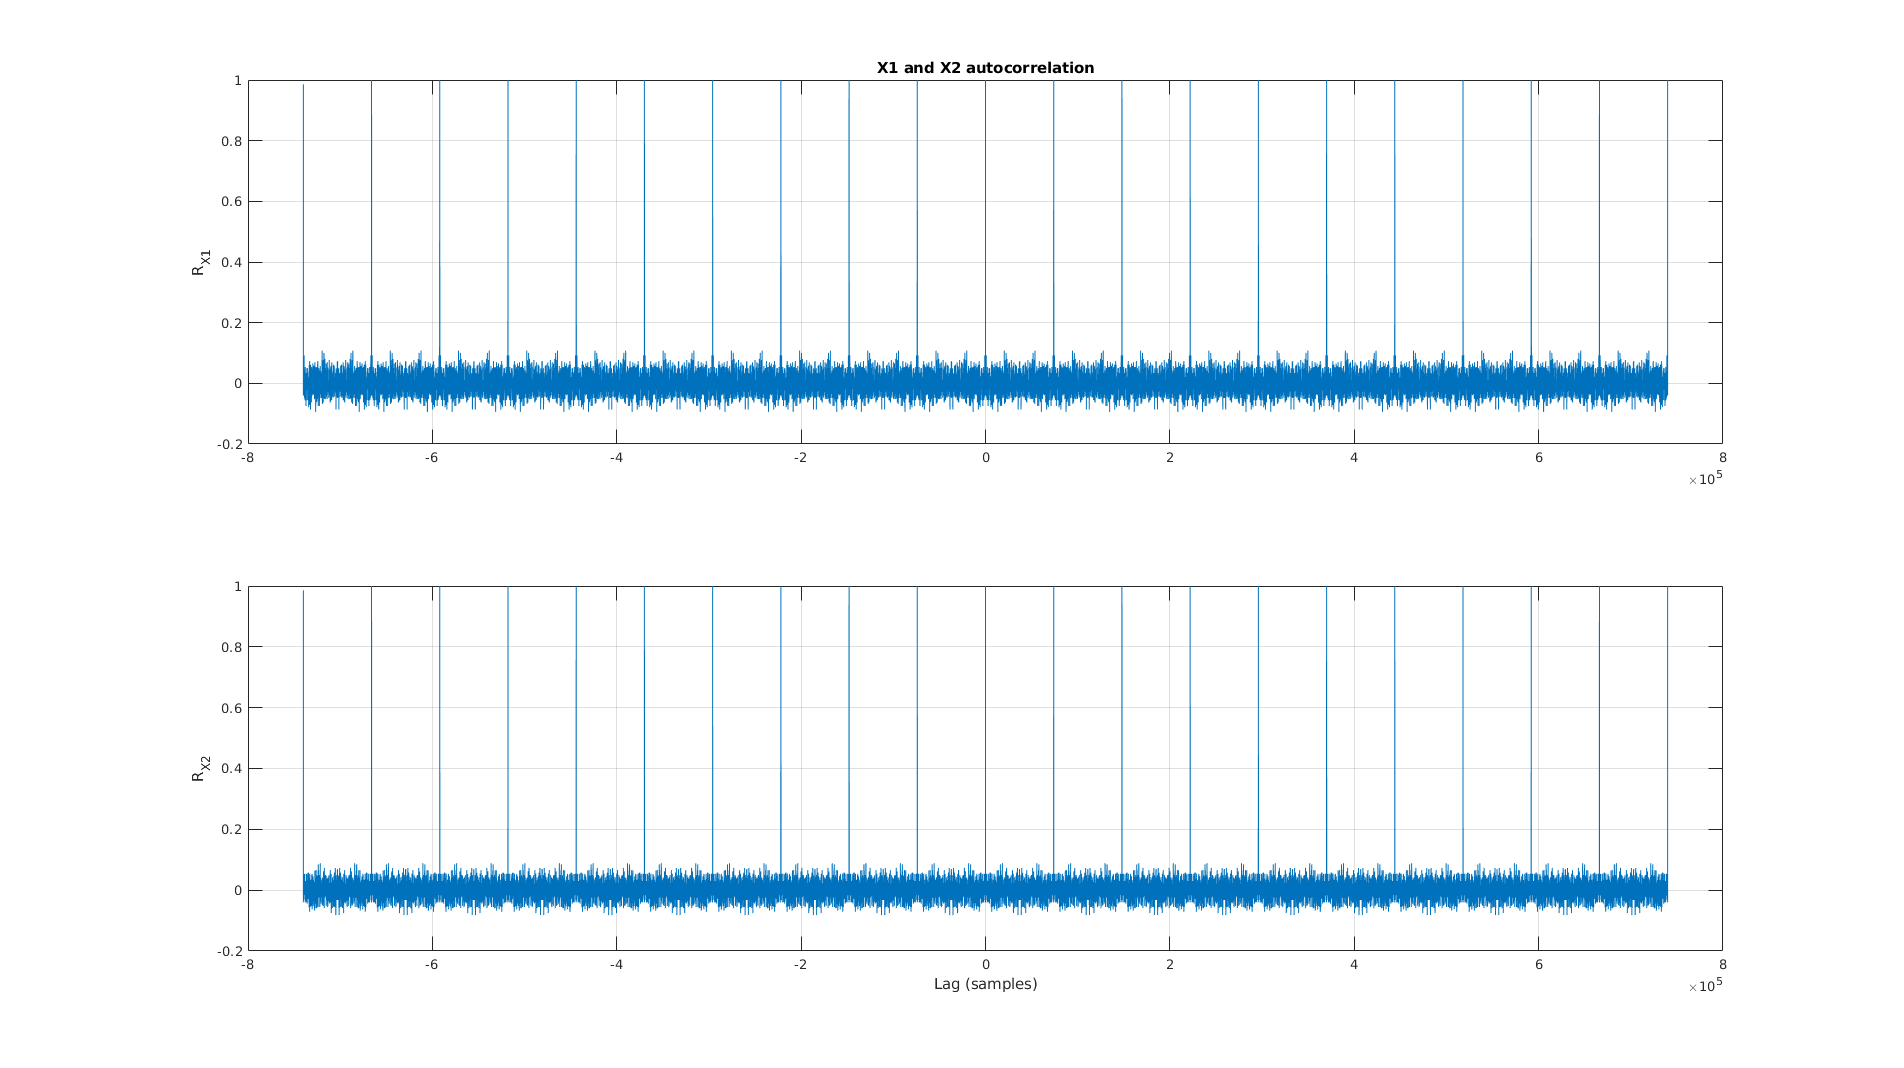
\includegraphics[width=0.9\textwidth]{figs/ex8_autocorr_pi.png}
	\caption{Autocorrelation of X1 and X2 for the 'pi' case.}
	\label{fig:ex8_autocorr_pi}
\end{figure}

\begin{figure}[H]
	\centering
	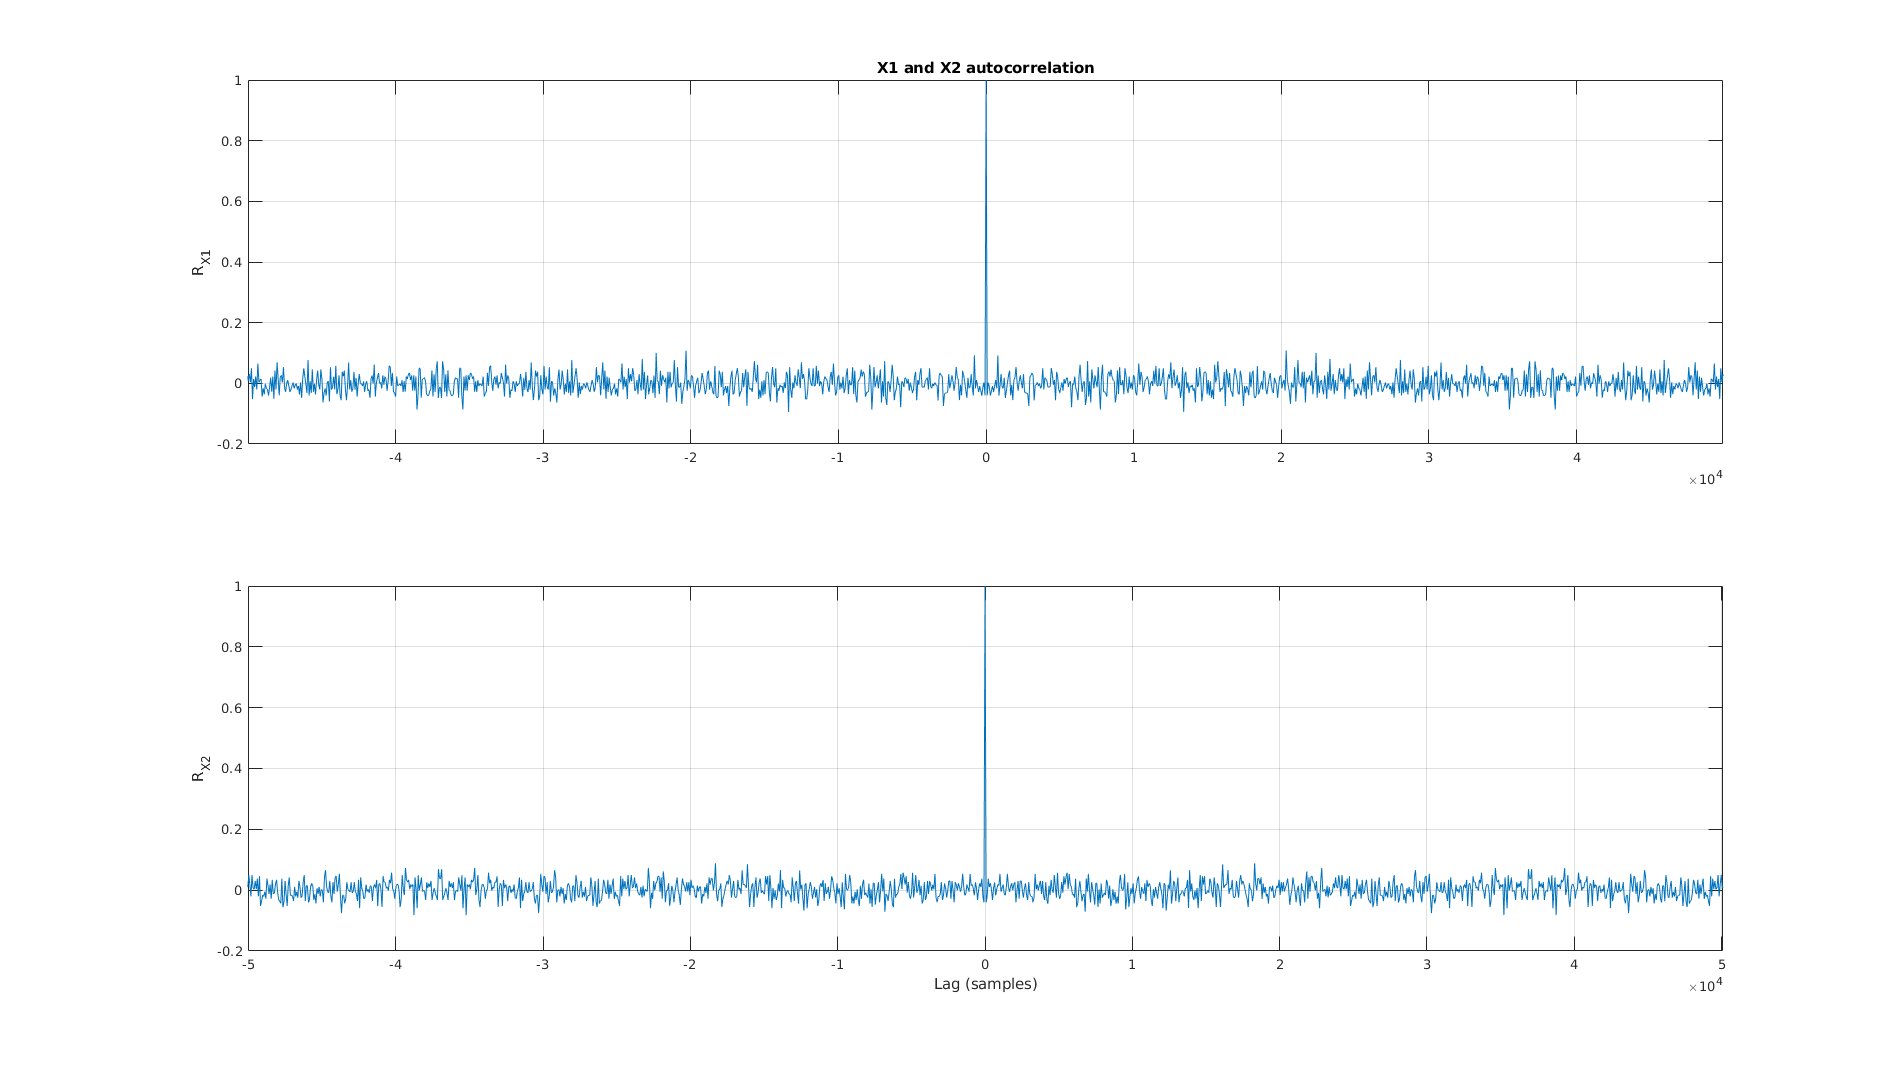
\includegraphics[width=0.9\textwidth]{figs/ex8_autocorr_zoomed_pi.png}
	\caption{Zoomed autocorrelation of X1 and X2 for the 'pi' case.}
	\label{fig:ex8_autocorr_zoomed_pi}
\end{figure}

The ratio of the maximum of $R_X(\tau)$ to the maximum of $R_{X1,X2}(\tau)$ is
10.12 for the case where we work with 'pi' method.

\begin{figure}[H]
	\centering
	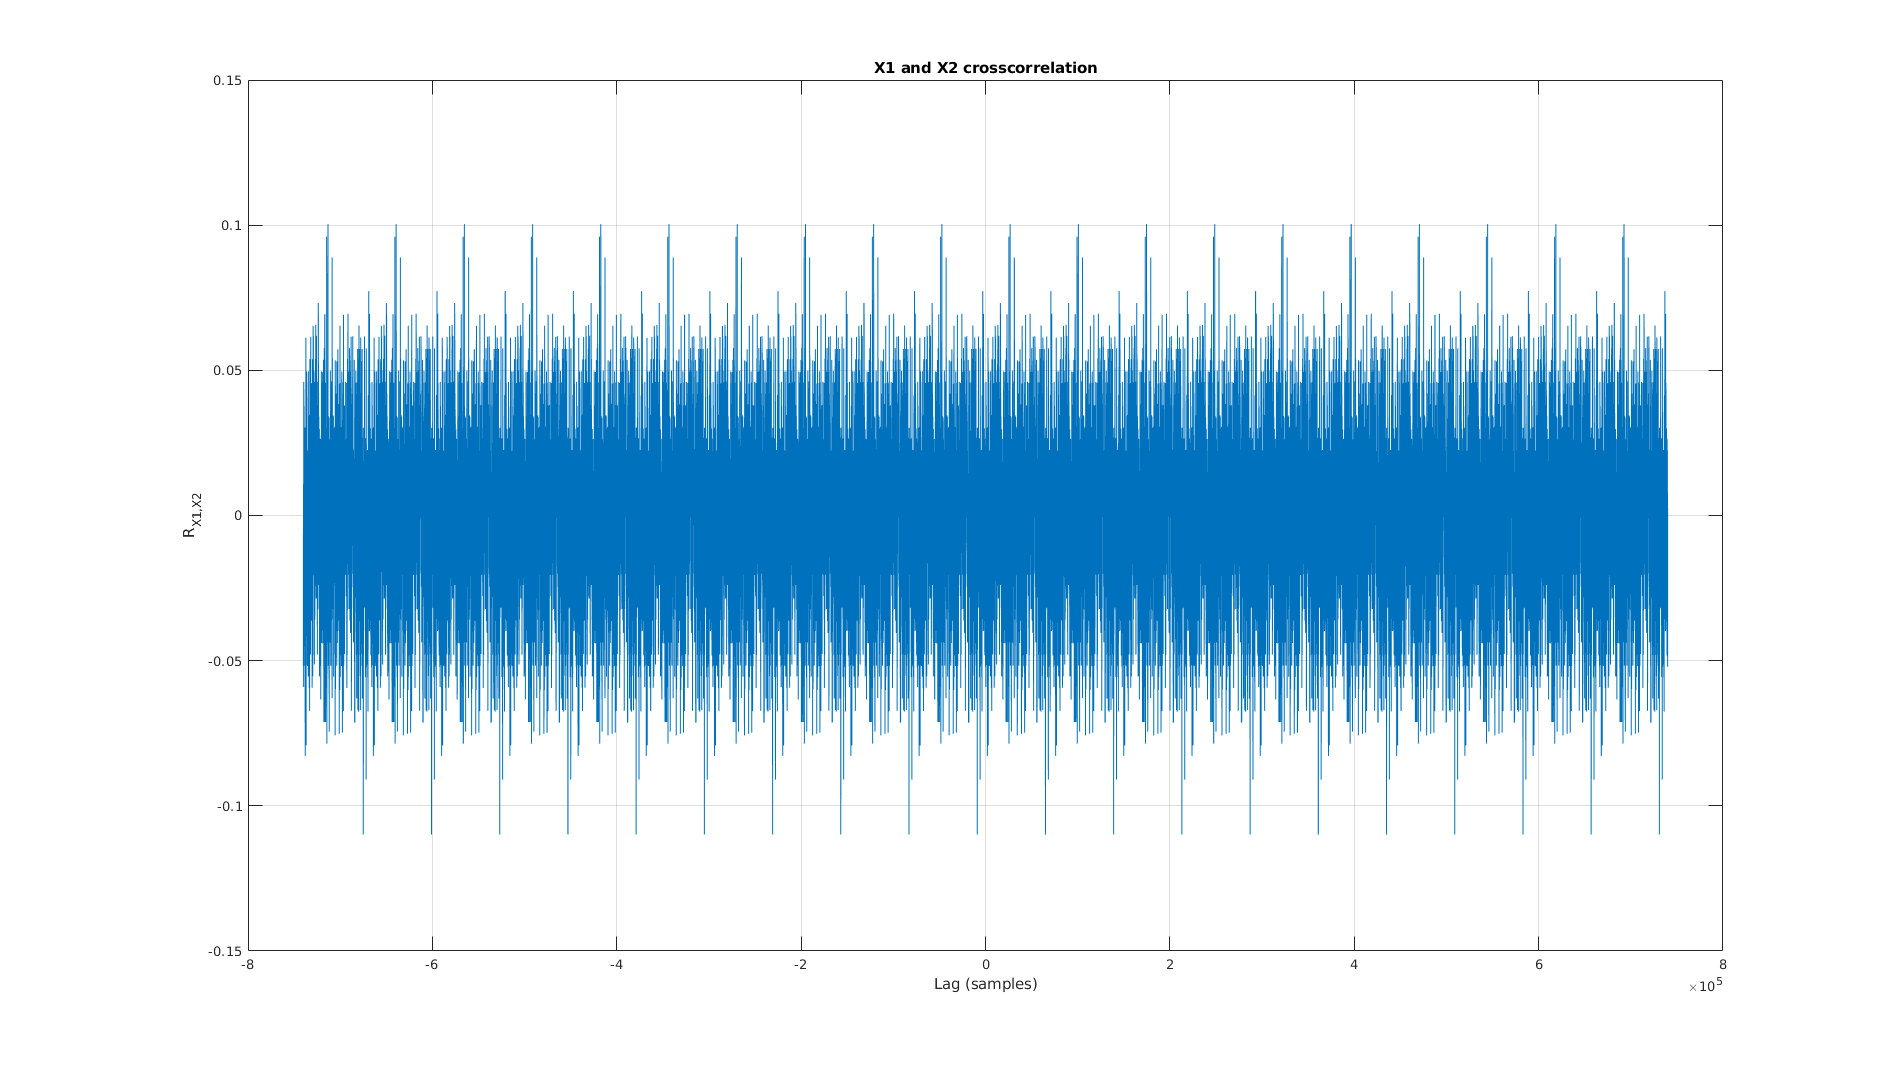
\includegraphics[width=0.9\textwidth]{figs/ex8_crosscorr_mseq.png}
	\caption{Crosscorrelation of X1 and X2 for the 'mseq' case.}
	\label{fig:ex8_crosscorr_mseq}
\end{figure}

\begin{figure}[H]
	\centering
	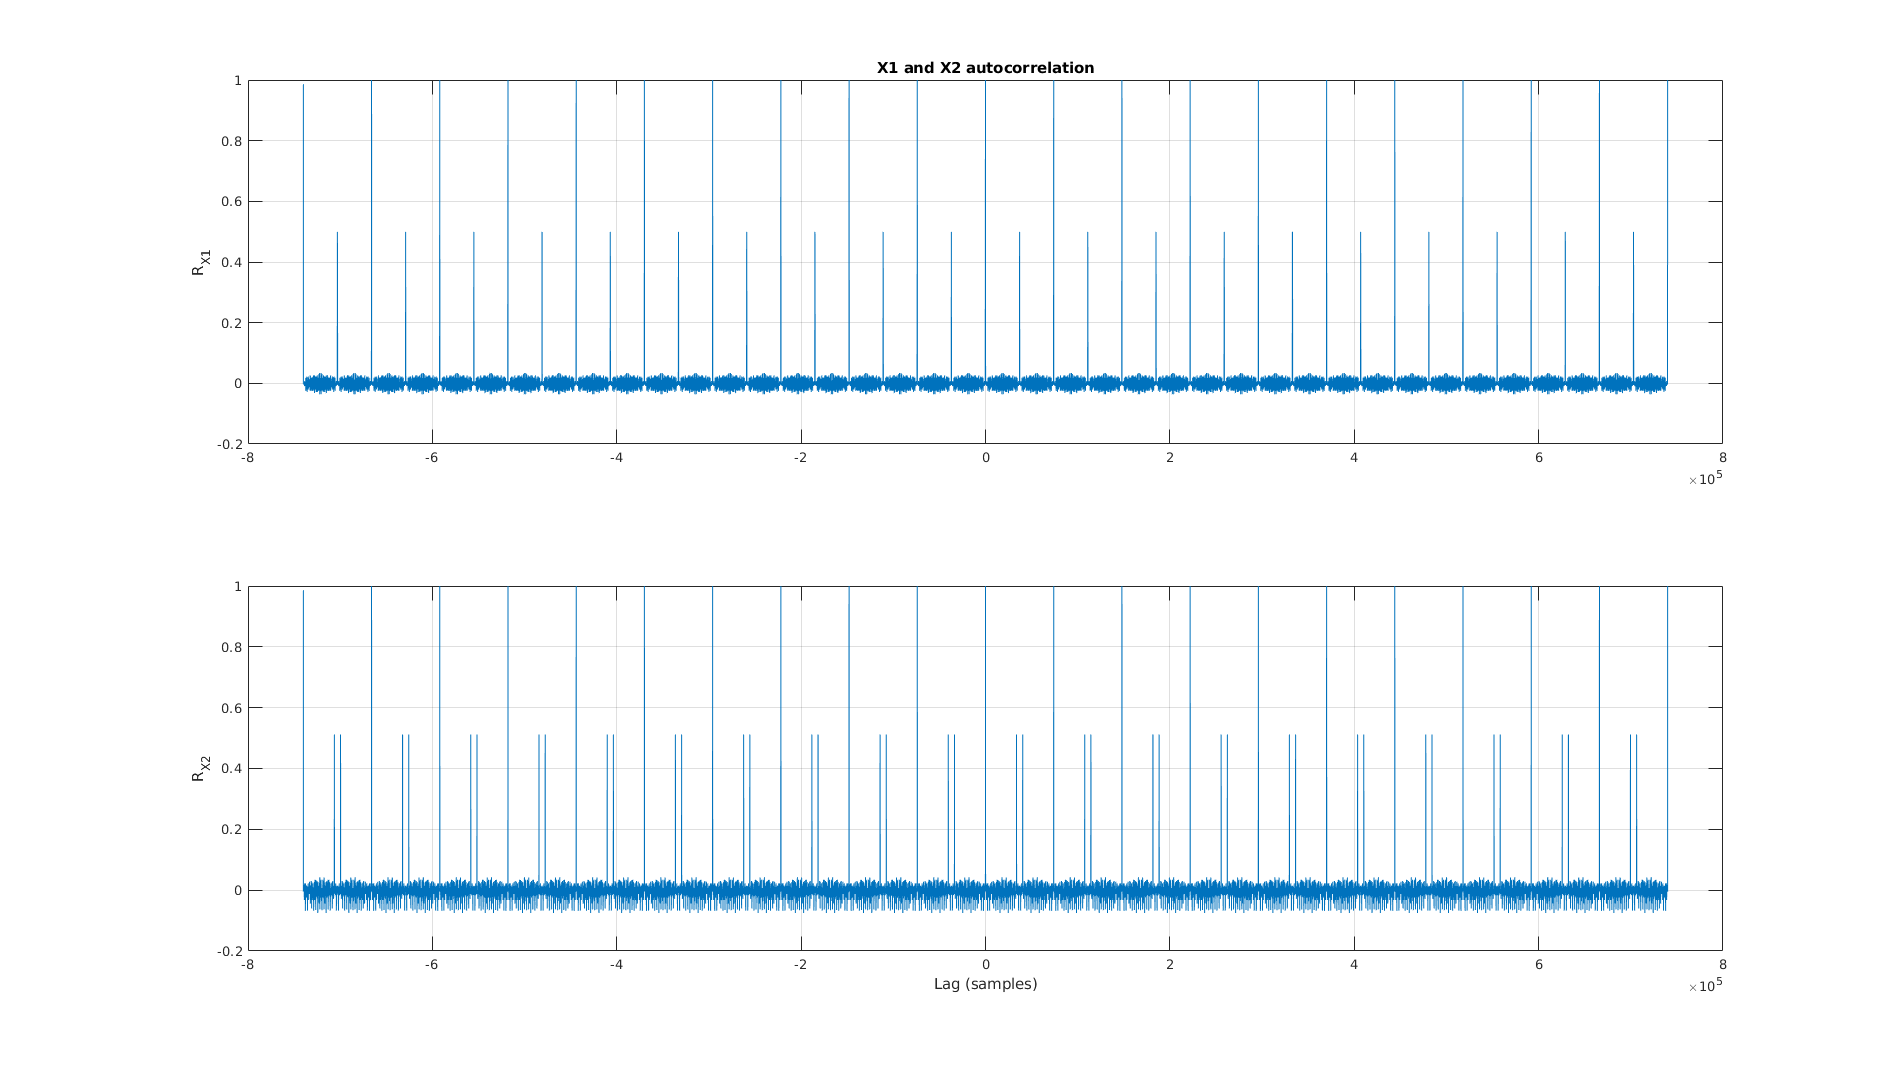
\includegraphics[width=0.9\textwidth]{figs/ex8_autocorr_mseq.png}
	\caption{Autocorrelation of X1 and X2 for the 'mseq' case.}
	\label{fig:ex8_autocorr_pi}
\end{figure}

\begin{figure}[H]
	\centering
	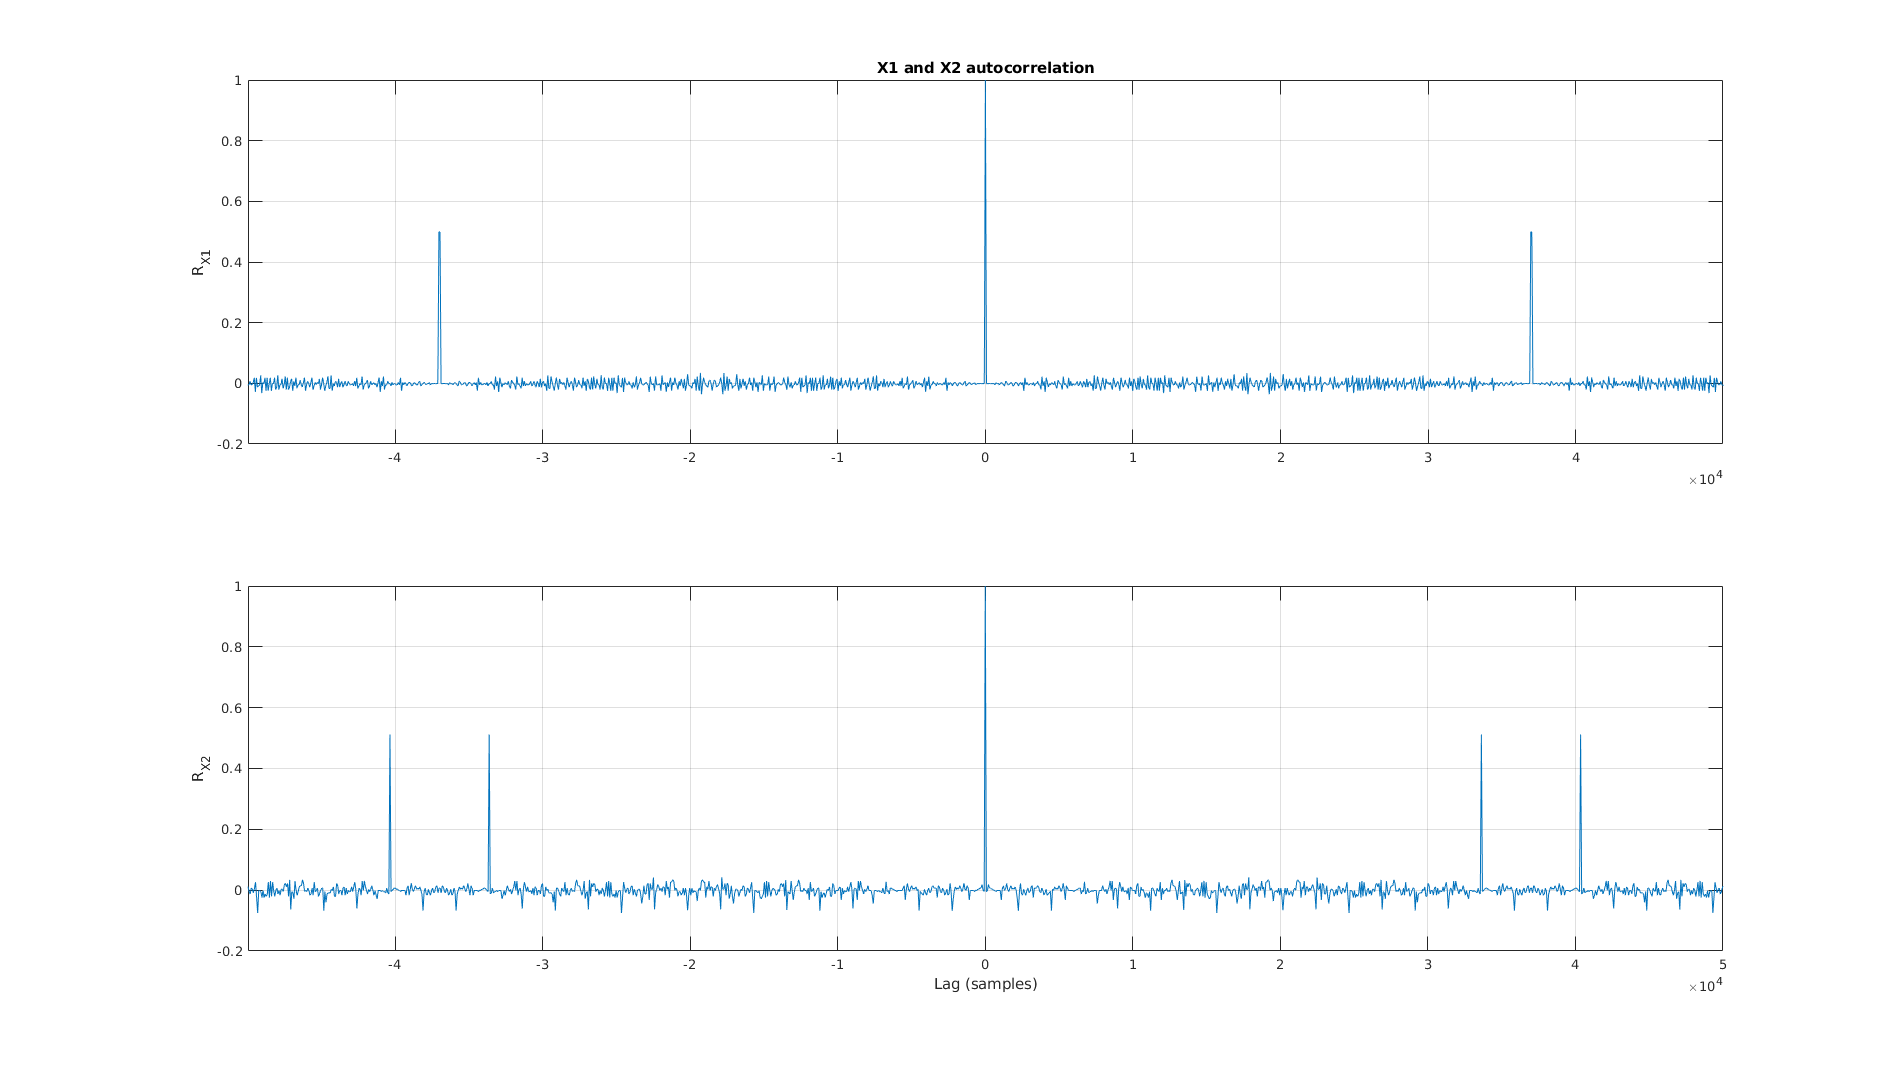
\includegraphics[width=0.9\textwidth]{figs/ex8_autocorr_zoomed_mseq.png}
	\caption{Zoomed autocorrelation of X1 and X2 for the 'mseq' case.}
	\label{fig:ex8_autocorr_zoomed_mseq}
\end{figure}

The ratio of the maximum of $R_X(\tau)$ to the maximum of $R_{X1,X2}(\tau)$ is
9.9659 for the case where we work with 'mseq' method.

Analyzing the graphs it's hard to conclude which method provides the best
cross-correlation properties. They all look very similar, showing values
concentrated below arround +-0.05 and spikes upto +-0.1. The ideal behavior we
are looking for is a cross-correlation equal to zero. Which would indicate that
no two signal could be confused because they are perfectly orthogonal.

The analysis of the autocorrelation is a little different. The 'rand' and 'pi'
methods look very similar. But the 'mseq' method is quite different. It has a
much lower floor, which it's closer to the ideal case we are looking for: the
Dirac delta. However, it presents smaller spikes to the sides. This could be
pretty bad because one could confuse this smaller peaks with the main peak and
consequently get an inaccurate range measurement due to pourly "locking" to the
local replica of the code. In addition to the aforementioned, the calculated
ratios show that the 'rand' method provides the greater relationship between
max autocorrelation and max cross-correlation, which is a desired property since
it means that there are more chances of correctly identifing and 'locking' to
the desired satellite's code. This result surprised me since I was expecting the
mseq to have the best properties.
